\section{问题三建模}
在问题三中,我们需要根据第一问中以获得的车辆相关信息,对目前为机械方案的红绿灯配时进行优化,在不同的子时间段进行适应性调节,设定更加合理的周期与配时。优化算法考虑Webster配时法和遗传算法。

此外还要在原有车辆信息基础上,利用优化后的时间数据,对车辆通行情况进行仿真模拟,重新统计得到优化后的基本信息。

基本假设:

(1)有车辆在行驶过程中,无突发事故影响正常行驶

(2)交通信号灯均按照配时方案正常工作

(3)忽略行人、非机动车的行动对车辆行驶的影响

\subsection{信息提取}

\subsubsection{相位方案}
信号相位指交通信号灯给各方向的车辆轮流分配通行权的信号显示,通过观察,现有四相位方案下右转车道基本保持通畅,因此考虑基于直行与左转绿灯的四相位优化方案。相位方案如下图\ref{fig:相位}所示:
\begin{figure}[h]
    \centering
    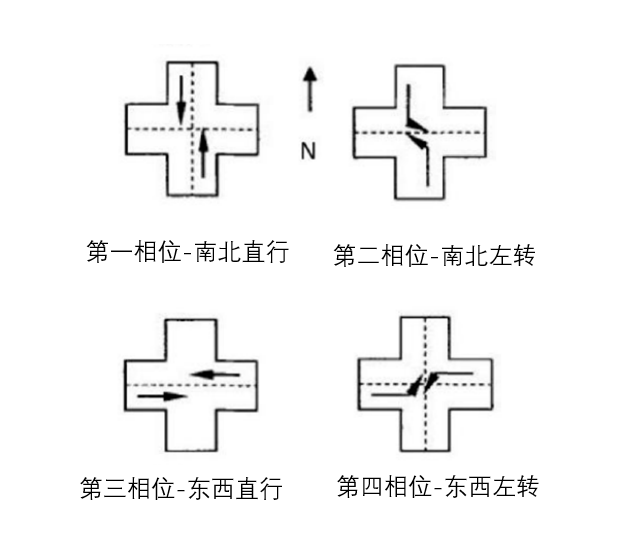
\includegraphics[scale=0.5]{figures/四相相位图.png}
    \caption{相位示意图}
    \label{fig:相位}
\end{figure}

\subsubsection{交通流量折算}
模型中用到多个关于车流量的变量,单位为pcu,指标准车当量数。对各种各样的实际车辆按《城市道路设计规范》中规定的折算系数折算系数换算成某种标准车型的当量交通量。数据中涉及到的车型对应折算比例为:小型车1.0,大客车、中型货车1.5,大型货车2.0。

\subsubsection{车道饱和流量校正}
基本饱和流量信息参考中国城市车道平均水平,记为$S_{ave}$直行车道1650pcu/h,右转车道1450pcu/h,左转车道1550pcu/h,按照道路信息进行宽度校正,转弯半径校正。宽度校正系数$f_w$在2.8m时为$0.4*(2.8-0.5)$,3.2m时为1。转弯半径校正系数$f_r$,依照提取出的转弯半径信息,在左转时为1,右转时为0.97。可得到实际车道饱和流量$S=S_{ave}*f_w*f_r$。

\subsection{现有方案分析}

\subsubsection{机械配时方案}
通过提取所给场景中的信号灯变化信息,提取出初始机械配时周期,东西方向全红灯(可右行)亮57秒,直行(可右转)绿灯亮30秒,黄灯亮3秒,左转(可右转)绿灯亮20秒,黄灯再亮3秒;南北方向全红灯亮56秒,仅直行绿灯亮23秒,黄灯亮3秒,左转(可右转)绿灯亮28秒,黄灯再亮3秒,该周期共113秒。东西方向全红灯开始时间与南北方向直行绿灯亮起时间保持一致,因此一周期内的全红时间为0。

\subsubsection{实际流量值}
为了有效分析各相位下不同行驶方向上的时间需求大小,依照现有进入时间等相关信息,经过缺失填补、流量折算、单位换算等步骤得到各周期四相位下的实际标准车流量值,以pcu/h为单位。选择相对应方向上较大的车辆通行数,得到表格数据与折线图。
\begin{figure}[H]
    \centering
    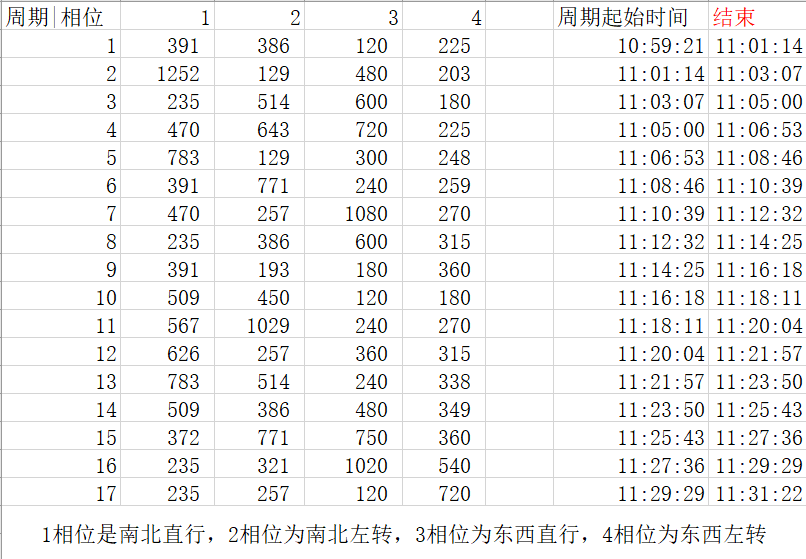
\includegraphics[scale=0.5]{figures/流量分周期图.png}
    \caption{流量分周期图}
    \label{fig:流量分周期图}
\end{figure}

\begin{figure}[H]
    \centering
    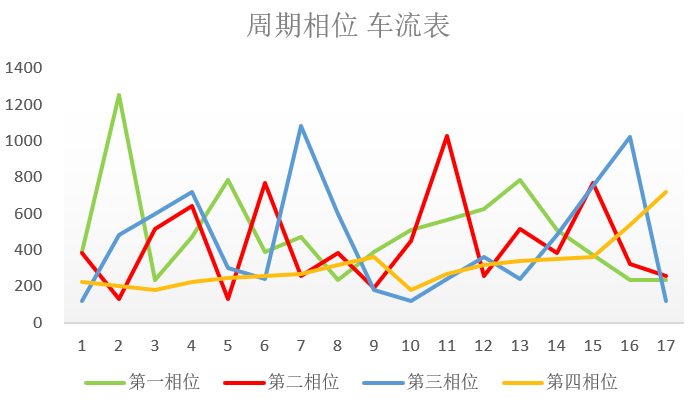
\includegraphics[scale=0.5]{figures/周期相位车流表.png}
    \caption{周期相位车流表}
    \label{fig:周期相位车流表}
\end{figure}
一二相位为南北通行方向,流通较大;三相位车流量大于趋于平稳的第四相位流通量。

\subsubsection{优化方案初设}
由于记录东西方向和南北方向的监控记录时间存在10秒左右的延误,因此我们考虑从基于同一周期的四相位车辆监控与配时优化。根据车辆信息进一步整理分析发现,目前车辆比较稀少,存在着明显的阻碍交通情况:南北/东西方向有车辆需要通行,可是南北/东西方向亮着红灯,而东西/南北方向亮着绿灯,不同时间段存在着不等长的道路空白期。故根据不同相位流通量大小特征,构成待优化的三组子时间段,利用优化方法分别进行优化。

第一子时间段:6,9-13周期,该情况下第一二相流通量明显高于三四相。

第二子时间段:3-4,7-8,14-17周期,该情况下第三相流通量较高。

第三子时间段:1-2,5周期,该情况下第一相流通量明显较高。

\subsection{目标函数建立}

\subsubsection{平均延误时间}
延误时间表示车辆受阻情况下通过岔路口的时间和正常行驶通过的时间差,由一致性延误$d_{u}$描述到达率为常数的延误和随机延误$d_{r}$此时到达率不为常数,两部分组成。计算方法分别如下:
\begin{equation}
    d_{ui}=\sum_{j} \frac{c\left(1-g_{i} / c\right)^{2}}{2\left(1-y_{i j}\right)}
\end{equation}
\begin{equation}
    d_{ri}=\sum_{j} \frac{y_{i j}^{2}}{2 q_{i j}\left(1-y_{i j}\right)}
\end{equation}
\begin{equation}
    d_{i}=d_{ui}+d_{ri}
\end{equation}
其中$i = 1,2,3,4$表示四个相位,$j=1,2,3,4$表示四个车道;$d_i$表示第i相位平均延误;$c$为周期长信号灯各色完整显示所花时间,这里为113s;$g_i$表示第i相位有效绿灯时长,$q_{ij}$表示第i相位第j车道进口当前流量值pcu/h;$y_{ij}$表示第i相位第j车道进口交通强度,即实际流量值和饱和流量值的比值。因此一周期内的平均延误为各相位延误加权平均值,计算公式为:$\sum_{i} d_i q_{i} /\sum_{i} q_{i}$,其中$q_{i}=\sum_{j} q_{ij}$。

\subsubsection{进入速度损失}
由于车辆停车的可能性与交通饱和率成反比,相关资料表明车辆的平均停车次数可由
\begin{equation}
    w_{i}=\sum_{j} 0.9 \frac{\left(c-g_{i}\right)}{1-y_{i j}}
\end{equation}
估计,因此对应第i相位所有进入车辆产生的平均速度$v_i$,通过实际计算采用$v_i'=v_i/10$作为速度加权因子,得到各相位速度损失加权平均值:$\sum_{i}v_i h_i q_{i} /\sum_{i} q_{i}$。

\subsubsection{通行能力}
通行能力用于表示车辆在有效绿灯时间通过停车线的数目,根据交通管理与控制标准计算方法求得
\begin{equation}
    z_{i}=\frac{s_{i} \times g_{i}}{c}
\end{equation}
$s_i$为第i条进口车道的饱和流量。在此基础上进行相位加权得:$\sum_{i} z_i q_{i} /\sum_{i} q_{i}$

\subsubsection{目标函数与约束条件}
为使车辆通过路口的平均速度最大,以延误时间最短,进入速度损失最小,通行能力最大为目标。利用罚函数的思想建立了如下目标函数
\begin{equation}
    \min _{X} f(X)=\sum_{i}( k_{i}^{1} d_{i}+k_{i}^{2} w_{i}-k_{i}^{3} z_{i})
\end{equation}
其中$k_{i}^{1}, k_{i}^{2}, k_{i}^{3}$系数设置参考\cite{顾怀中1998交叉口交通信号配时模拟退火全局优化算法},对应计算方法为$k_{i}^{1}=2(1.0-Y) \times \sqrt[7]{s_{i}}$,$ k_{i}^{2}=\sqrt[7]{s_{i}} \times \frac{1.0-Y}{0.9}$,$k_{i}^{3}=2 Y \times \frac{c}{3600}$。其中$Y=\sum \operatorname{max}y_{ij}$。

约束条件为周期时间约束,饱和度约束等,具体表达式如下:
$$C_{\min } \leqslant C \leqslant C_{\max }$$
$$\sum_{i} (g_{i}+t_{l})=C$$
$$0.7 \leqslant \frac{y_{i} c}{g_{i}} \leqslant 0.9,1 \leqslant i \leqslant n$$
$$g_{i} \in Z^{+}, 1 \leqslant i \leqslant n$$
0.7用来避免在饱和度过小,即通行能力远大于需求,增加车辆阻碍,0.9用来避免饱和度过大而造成堵塞。$t_l$表示每相损失时间,由启动损失时间$t_{l1}$和清尾损失$t_{l2}$分组成,停车等待的车辆在绿灯开始时不能立即提高速度,存在时间损失$t_{l1}$,一般为2s,清尾损失$t_{l2}$表示黄灯时间,这里为3s。故,$t_l=5s$。

\subsection{优化算法与结果展示}

\subsubsection{Webster时配算法}
韦伯斯特(Webster)算法以降低交叉口车辆延误为目标,进行配时优化的经典算法。通过大量现场交通观察,结合排队论和计算机模拟得出的算法。在单点信号配时、平峰路口优化方面效果良好,与文中所示情况相符。运用近似解法,得到最佳周期时长为
\begin{equation}
    c_{0}=\frac{1.5 L+5}{1-Y}
\end{equation}
最佳有效绿灯时长为
\begin{equation}
    g_{i}=(c_{0}-t_l*4)\frac{y_i}{\sum_{i} y_{i}}
\end{equation}

\subsubsection{遗传算法}
遗传算法是一种效率较高的参数寻找最优解的算法,参考仿生原理快速搜索解空间,因此适用于该问题关于交通系统时间配置的优化问题。
算法基本步骤如下:(1)设置如种群大小、交叉概率等的基本参数;(2) 对问题进行实数编码,用解数据表示基因型串结构数据;(3)随机生成串行结构初值作为初始种群;(4)基于动态函数惩罚法来构造适应度函数:$F(x)=\frac{1}{\varepsilon+f(x)}$;(5) 适应度比例的选择采用轮盘赌方法;(6)采用取自$[0,1]$的随机数的实数交叉法;(7)采用非均匀变异对原有基因进行小范围扰动;(8)记录结果,进行判断是否需要进行下一次迭代。
\textcolor{white}{\cite{孙超2008城市单点交叉口的信号配时优化研究} \cite{顾怀中1998交叉口交通信号配时模拟退火全局优化算法}\cite{张力2014结合遗传算法的混合式蚁群单点交叉口信号配时算法}\cite{慕飞飞2015基于遗传算法的单点交叉口信号配时优化}\cite{颜艳霞2006单点交叉口信号实时配时模型及蚂蚁算法}\cite{2016You}}

\subsubsection{优化配时方案}
通过数据计算可知,现有配时对应平均延误较大,主要原因在于相位交通流量与对应时间存在差距。

利用已有信息结合Webster算法,进行优化。相位启动损失为2s,黄灯时长保持为3s,计算得出 不同方案最佳周期与各相位有效绿灯时长。如下表\ref{fig:Webster}所示:

\begin{figure}[h]
    \centering
    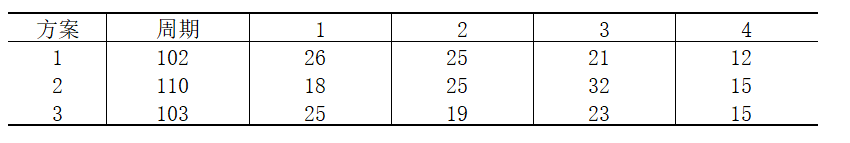
\includegraphics[scale=0.7]{figures/Webster.png}
    \caption{Webster}
    \label{fig:Webster}
\end{figure}

遗传算法中的设定最小信号周期为60s,最大信号周期为120s,最大有效绿灯时长为30s,最小为10s。参数设置如下:最大遗传代数为500,初始种群大小为100,交叉率为0.8,染色体长为5,变异率为0.01。结果如\ref{fig:遗传算法}所示。

\begin{figure}[h]
    \centering
    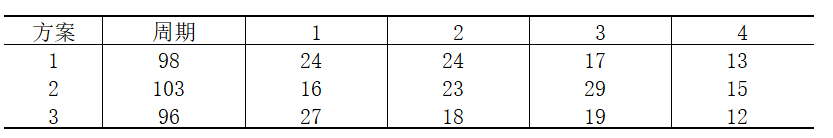
\includegraphics[scale=0.7]{figures/遗传算法.png}
    \caption{遗传算法}
    \label{fig:遗传算法}
\end{figure}

\subsection{模拟实验}

\subsubsection{车流模拟}
在模拟试验中,车辆以表一中的车辆进入相关信息编制车辆行驶算法,使车辆在红绿灯相位在对应的车道执行停车等待,启动离开的行驶动作,所有车辆在黄灯开始时不超越停车线。在此基础上添加动态算法,防止车辆与车辆之间的碰撞。

\subsubsection{优化结果对比}
从计算机视觉的视角,一张图片我们需要考虑多个坐标系,最终结果如图\ref{fig:优化对比}所示。通过表格所显示的优化指标结果可以看出,经典的Webster算法以及遗传算法均对现有方案进行了改进。其中遗传算法效果更佳,该方案能更高效适配已知车辆进入信息,使得通行速度得以提高。

\begin{figure}[h]
    \centering
    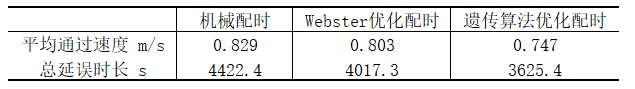
\includegraphics[scale=0.7]{figures/优化对比.png}
    \caption{优化对比}
    \label{fig:优化对比}
\end{figure}
